%\documentclass{article}
\usepackage[utf8]{inputenc}
\pagenumbering{gobble}
\title{Diario del progetto}
%\date{A.A. 2022/22}
\date {}
%\usepackage{blindtext}\usepackage[a4paper, total={6in, 8in}]{geometry}
\usepackage{geometry}
\usepackage{graphicx}
\graphicspath{ {./images/} }
\geometry{
    a4paper,
    total={170mm,257mm},
    left=20mm,
    top=20mm,
}
\usepackage{pdflscape}
%Definizione Variabili
\newcommand\uno{Scrum Master (Alessia Crimaldi), Dev 1 (Alessio Arcara), Dev 2 (Matteo Sacco).}
\newcommand\unoP{Product Owner (Davide Fermi), }
\newcommand\due{Scrum Master (Davide Fermi), Dev 1 (Alessia Crimaldi), Dev 2 (Alessio Arcara).}
\newcommand\dueP{Product Owner (Matteo Sacco), }
\newcommand\tre{Scrum Master (Matteo Sacco), Dev 1 (Davide Fermi), Dev 2 (Alessia Crimaldi).}
\newcommand\treP{Product Owner (Alessio Arcara), }


\begin{document}
    \begin{landscape}

        \maketitle

        \section{SPRINT 01}

        \begin{itemize}
            \item Inizio sprint: \textit{08/01/2023}
            \item Fine sprint: \textit{14/01/2023}
        \end{itemize}

        \begin{itemize}
            \item \textbf{Sprint Goal (SG):}
            \begin{indent}
                \newline Permettere ad un visitatore di utilizzare tutte le funzionalita' base dell'app, ossia di avere una corretta ed efficace importazione e gestione del catalogo carte con le relative ricerche e visualizzazione dei dettagli della carta.
            \end{indent}
        \end{itemize}

        \begin{itemize}
            \item \textbf{Ruoli:}
            \newline \textbf{Product Owner:} Davide Fermi
            \newline \textbf{Scrum Master:} Alessia Crimaldi
            \newline \textbf{Development team:} Alessio Arcara, Matteo Sacco
        \end{itemize}
        \vspace{5mm} %5mm vertical space
        \subsection{Sprint Planning (S01)}
        \item \textbf{Data:} 08/01/2023
        \newline \textbf{Durata:} 95 min.
        \newline \textbf{Partecipanti:} \unoP \uno
        \\
        \newline La riunione inizia con la presentazione da parte del PO del Product Backlog, che ha introdotto le user stories e con le relative priorità. Viene proposto dallo Scrum Master di utilizzare il metodo \"Poker Planning\" per stablire gli story points per ogni UC e viene selezionato uno strumento online per facilitare l'utilizzo del metodo. Viene concordato dal team, tra le scale disponibili, di utilizzare la sequenza di Fibonacci modificata (0  1/2  1  2  3  5  8  13  20  40  100  ?  -tazzina di caffè-). Si sottolinea come il Poker Plain ha permesso al team di lavorare insieme e dinamicamente, confrontandosi e discutendo, per giungere a una decisione condivisa, nonostante che le opinioni individuali iniziali fossero a volte distanti. Successivamente si è passato a stimare l'effort per ogni user stories per poi definire l'effort totale settiminale per lo sviluppo. E' stato successivamente popolato lo Sprint Backlog a cura degli sviluppatori e dello SM, fino al raggiungimento dell'effort totale precedentemente stimato. Ogni singolo UC presente nello Sprint Backlog è stato successivamente raffinato in tasks di sviluppo, per ognuno dei quali è stato stimato un effort.

        \newpage
        \subsection{Stato board dopo lo Sprint Planning (S01):}
        \begin{itemize}
            \small
            \def\arraystretch{2}%
            \begin{tabular}{ | p{6cm} | p{3.2cm} | p{7.8cm} | p{3cm} | p{2.8cm}| }
                \hline
                \textbf{UC raffinati}
                & \textbf{Product Backlog}
                & \textbf{Sprint Backlog}
                & \textbf{Sprint In progress}
                & \textbf{Sprint Done} \\
                \hline
                \textbf{UC01:} Come visitatore voglio selezionare un gioco e vedere l'elenco di tutte le sue carte
                & & \textbf{Task1 [UC01]\#2:} Creare il modello per le carte di tutti i giochi & & \\
                \hline
                \textbf{UC02:} Come visitatore voglio poter fare delle ricerche per vedere un elenco di carte filtrato
                & & \textbf{Task2 [UC01]\#3:} Importare dai JSON le carte dei giochi & & \\
                \hline
                \textbf{UC03:} Come visitatore voglio selezionare una carta e vederne i dettagli
                & & \textbf{Task3 [UC01]\#4:} Inizializzare il DB con i JSON caricati & & \\
                \hline
                & & \textbf{Task4 [UC01]\#5:} Creare RemoteService per fetch delle carte di quel gioco & & \\
                \hline
                & & \textbf{Task5 [UC01]\#6:} Creare HomeView per la visualizzazione delle carte & & \\
                \hline
                & & \textbf{Task6 [UC01]\#7:} Creare Composite Card per la visualizzazione carta & & \\
                \hline
                & & \textbf{Task1 [UC02]\#10:} Creare filtri specifici di quel gioco & & \\
                \hline
                & & \textbf{Task2 [UC02]\#11:} Filtrare l'array delle carte in base ai filtri specificati & & \\
                \hline
                & & \textbf{Task3 [UC02]\#12:} Rimuovere dalla pagina HomeView le carte che non corrispondono ai filtri & & \\
                \hline
                & & \textbf{Task1 [UC03]\#14:} Creazione CardPlace & & \\
                \hline
                & & \textbf{Task2 [UC03]\#15:} Connessione RemoteService FetchCard nel caso l'assunzione sia errata & & \\
                \hline
                & & \textbf{Task3 [UC03]\#16:} Creazione CardView e popolamento delle informazioni & & \\
                \hline
                & & \textbf{Task4 [UC03]\#17:} Gestione del cambio di pagina da HomeView a CardView & & \\
                \hline
            \end{tabular}
        \end{itemize}
        \normalsize

        \newpage
        \subsection{Daily Scrum (S01):}
        \begin{itemize}
            \item \textbf{Data:} 09/01/2023
            \newline \textbf{Durata:} 15 min.
            \newline \textbf{Partecipanti:} Scrum Master (Alessia Crimaldi), Dev 1 (Alessio Arcara).
            \newline \textbf{Percezione attuale dello SG:} Positiva (Dev 1)
        \end{itemize}
        \begin{itemize}
            \item \textbf{Data:} 10/01/2023
            \newline \textbf{Durata:} 15 min.
            \newline \textbf{Partecipanti:} \uno
            \newline \textbf{Percezione attuale dello SG:} Negativa (Dev 1), Positiva (Dev 2)
        \end{itemize}
        \begin{itemize}
            \item \textbf{Data:} 11/01/2023
            \newline \textbf{Durata:} 15 min.
            \newline \textbf{Partecipanti:} \uno
            \newline \textbf{Percezione attuale dello SG:} Negativa (Dev 1), Negativa (Dev 2)
        \end{itemize}
        \begin{itemize}
            \item \textbf{Data:} 12/01/2023
            \newline \textbf{Durata:} 15 min.
            \newline \textbf{Partecipanti:} \uno
            \newline \textbf{Percezione attuale dello SG:} Negativa (Dev 1), Negativa (Dev 2)
        \end{itemize}
        \begin{itemize}
            \item \textbf{Data:} 13/01/2023
            \newline \textbf{Durata:} 12 min.
            \newline \textbf{Partecipanti:} \uno
            \newline \textbf{Percezione attuale dello SG:} Negativa (Dev 1), Negativa (Dev 2)
        \end{itemize}
        \begin{itemize}
            \item \textbf{Data:} 14/01/2023
            \newline \textbf{Durata:} 10 min.
            \newline \textbf{Partecipanti:} \uno
            \newline \textbf{Percezione attuale dello SG:} Negativa (Dev 1), Negativa (Dev 2)
        \end{itemize}
        \\
        \newline
        \newline \textbf{Note:} Si è cercato di mantenere i daily entro i 10 minuti, nella quale il team di sviluppo, condotti dallo Scrum Master, nella quale gli sviluppatori espongono quanto fatto, quanto hanno in progetto di fare e i principali problemi riscontrati. Al termine, lo Scrum master chiede una percezione dello Sprint Goal e mostra il BurnDown chart aggiornato.
        \newpage
        \subsection{Stato Board finale (S01):}
        \small
        \def\arraystretch{2}%
        \begin{tabular}{ | p{5cm} | p{3cm} | p{5cm} | p{5cm} | p{5cm}| }
            %begin{tabular}{p{0.1\textwidth}p{0.8\textwidth}p{0.1\textwidth}p{0.8\textwidth}p{0.8\textwidth}}
            \hline
            \textbf{UC raffinati}
            & \textbf{Product Backlog}
            & \textbf{Sprint Backlog}
            & \textbf{Sprint In progress}
            & \textbf{Sprint Done} \\
            \hline
            \textbf{UC01:} Come visitatore voglio selezionare un gioco e vedere l'elenco di tutte le sue carte
            & & \textbf{Task1 [UC03]\#14:} Creazione CardPlace
            & \textbf{Task2 [UC02]\#11:} Filtrare l'array delle carte in base ai filtri specificati
            & \textbf{Task1 [UC01]\#2:} Creare il modello per le carte di tutti i giochi \\
            \hline
            \textbf{UC02:} Come visitatore voglio poter fare delle ricerche per vedere un elenco di carte filtrato
            & & \textbf{Task2 [UC03]\#15:} Connessione RemoteService FetchCard nel caso l'assunzione sia errata
            & \textbf{Task3 [UC02]\#12:} Rimuovere dalla pagina HomeView le carte che non corrispondono ai filtri
            & \textbf{Task4 [UC01]\#5:} Creare RemoteService per fetch delle carte di quel gioco \\
            \hline
            \textbf{UC03:} Come visitatore voglio selezionare una carta e vederne i dettagli
            & & \textbf{Task3 [UC03]\#16:} Creazione CardView e popolamento delle informazioni
            & \textbf{Task6 [UC01]\#7:} Creare Composite Card per la visualizzazione carta
            & \textbf{Task5 [UC01]\#6:} Creare HomeView per la visualizzazione delle carte \\
            \hline
            & & \textbf{Task4 [UC03]\#17:} Gestione del cambio di pagina da HomeView a CardView
            & & \textbf{Task2 [UC01]\#3:} Importare dai JSON le carte dei giochi \\
            \hline
            & & & & \textbf{Task1 [UC02]\#10:} Creare filtri specifici di quel gioco  \\
            \hline
            & & & & \textbf{Task3 [UC01]\#4:} Inizializzare il DB con i JSON caricati \\
            \hline
        \end{tabular}
        \normalsize
        \newpage
        \subsection{Sprint Review (S01):}
        \begin{itemize}
            \item \textbf{Data:} 15/01/2023
            \newline \textbf{Durata:} 105 min.
            \newline \textbf{Partecipanti:} \unoP \uno
            \newline
            \newline I developers mostrano al PO una demo di quanto prodotto. Si evidenzia come non sia stato possibile sviluppare tutte le funzioni richieste dallo Sprint Goal. Si analizzano quindi le principali cause che hanno portato a questo problema, evidenziando come il framework GWT abbia portato della complessità nell'impementazione. Il PO decide quindi che non ci sono le condizioni sufficienti per procedere ad un rilascio, comprendendo le difficoltà riscontrate, ma chiedendo uno sforzo maggiore nello sprint successivo per poter raggiungere un prodotto rilasciabile. Non vengono evidenziati particolari problematiche di collaborazione e comunicazione all'interno del team.

            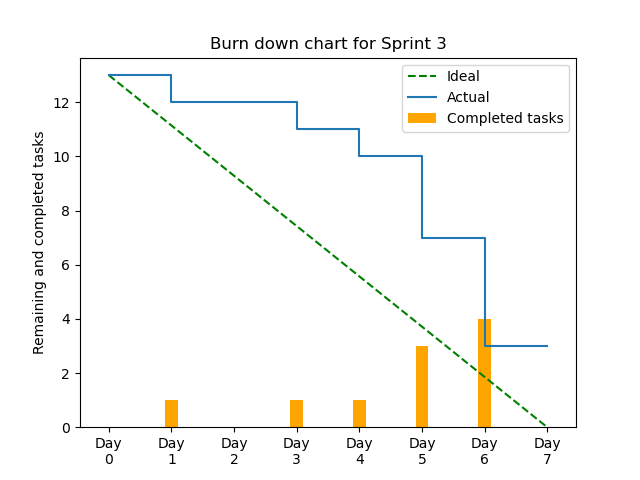
\includegraphics[scale=0.8]{Sprint03_BurnDownChart}
            --- METTERE QUELLO CORRETTO!!! ---

        \end{itemize}
        \newpage
        \subsection{Sprint Retrospective (S01):}
        \begin{itemize}
            \item \textbf{Data:} 15/01/2023
            \newline \textbf{Durata:} 70 min.
            \newline \textbf{Partecipanti:} \unoP \uno
            \newline
            \newline Lo Scrum Master chiede a tutti i membri di evidenziare gli aspetti positivi dello sprint appena concluso. Si riconosce come il lavoro di formazione durante la fase di inception abbia reso più veloce lo sviluppo, ma non abbastanza. Per quanto riguarda gli aspetti negativi, emerge, oltre a quanto già discusso nella review, che nonostante la percezione sia quasi da subito parsa negativa, non è stata applicata nessuna azione correttiva. Si decide quindi per il futuro, qualora si ripresentasse una situazione simile, di richiedere un confronto con il Product Owner e valutare se sia necessario rivedere lo Sprint Backlog, nel tentativo di migliorare dinamicamente il flusso di lavoro.
        \end{itemize}

        \newpage

        \section{SPRINT 02}

        \begin{itemize}
            \item Inizio sprint: \textit{15/01/2023}
            \item Fine sprint: \textit{22/01/2023}
        \end{itemize}

        \begin{itemize}
            \item \textbf{Sprint Goal (SG):}
            \begin{indent}
                \newline Permettere ad un visitatore di autenticarsi come utente e permettere ad un visitatore di effettuare una ricerca di carte dal catalogo potendo applicanre dei filtri.
            \end{indent}
        \end{itemize}

        \begin{itemize}
            \item \textbf{Ruoli:}
            \newline \textbf{Product Owner:} Matteo Sacco
            \newline \textbf{Scrum Master:} Davide Fermi
            \newline \textbf{Development team:} Alessio Arcara, Alessia Crimaldi
        \end{itemize}
        \vspace{5mm}
        \subsection{Sprint Planning (S02)}
        \begin{itemize}
            \item \textbf{Data:} 15/01/2023
            \newline \textbf{Durata:} 85 min.
            \newline \textbf{Partecipanti:} \dueP \due
            \\
            \newline Il Product Owner prensenta il Product Backlog aggiornato, descrivendo dettagliatamente gli UC presenti. Lo Scrum Master introduce il Poker Plain e vengono quindi assegnati gli story points dinamicamente e in maniera condivisa.  Il team stima l'effort per ogni user story e successivamente l'effort totale settimanale disponibile. Gli use cases vengono quindi inseriti nello Sprint Backlog, fino al raggiungimento dell'effort disponibile.  Gli sviluppatori effettuano la suddivisione dei singoli UC in task più dettagliati, per una maggiore comprensione e pianificazione. Lo Scrum master concorda con il team la pianificazione dei daily e li inserisce a calendario.
        \end{itemize}

        \newpage
        \subsection{Stato board dopo lo Sprint Planning (S02):}
        \begin{itemize}
            \small
            \def\arraystretch{2}%
            \begin{tabular}{ | p{6cm} | p{3.2cm} | p{7.8cm} | p{3.6cm} | p{2.2cm}| }
                \hline
                \textbf{UC raffinati}
                & \textbf{Product Backlog}
                & \textbf{Sprint Backlog}
                & \textbf{Sprint In progress}
                & \textbf{Sprint Done} \\
                \hline
                \hline
                \textbf{UC03:}  Come visitatore voglio selezionare una carta e vederne i dettagli
                & & \textbf{Task1 [UC03]\#14:} Creazione CardPlace & \textbf{Task2 [UC02]\#11:} Filtrare l'array delle carte in base ai filtri specificati   & \\
                \hline
                \textbf{UC04:}  Come utente voglio potermi autenticare per gestire i miei mazzi di carte
                &  & \textbf{Task2 [UC03]\#15:} Connessione RemoteService FetchCard nel caso l'assunzione sia errata &  \textbf{Task3 [UC02]\#12:} Rimuovere dalla pagina HomeView le carte che non corrispondono ai filtri & \\
                \hline
                \textbf{UC05:}  Come utente voglio poter aggiungere le mie carte reali al mazzo delle possedute
                &  & \textbf{Task3 [UC03]\#16:} Creazione CardView e popolamento delle informazioni  & \textbf{Task6 [UC01]\#7:}  Creare Composite Card per la visualizzazione carta &\\
                \hline
                & & \textbf{Task4 [UC03]\#17:} Gestione del cambio di pagina da HomeView a CardView & & \\
                \hline
                & & \textbf{Task1 [UC04]\#32:} Creare Authentication view per Login/registrazione  & & \\
                \hline
                & & \textbf{Task2 [UC04]\#33:} Creare RPC SignUp & & \\
                \hline
                & & \textbf{Task3 [UC04]\#34:} Creare RPC SignIn  & & \\
                \hline
                & & \textbf{Task4 [UC04]\#35:} Gestire la sessione  & & \\
                \hline
                & & \textbf{Task1 [UC05]\#36:} Creare modello per strutturare i mazzi predefiniti (possedute/desiderate) e il loro contenuto  & & \\
                \hline
                & & \textbf{Task2 [UC05]\#54:} Creare mappa dei mazzi su MapDB  & & \\

                \hline
                & & --- continua --- & & \\
                \hline
            \end{tabular}
            \newpage

            \begin{tabular}{ | p{6cm} | p{3.2cm} | p{7.8cm} | p{3.6cm} | p{2.2cm}| }
                \hline
                \textbf{UC raffinati}
                & \textbf{Product Backlog}
                & \textbf{Sprint Backlog}
                & \textbf{Sprint In progress}
                & \textbf{Sprint Done} \\
                \hline
                \hline
                & & \textbf{Task3 [UC05]\#63:} Creare metodo statico in AuthService per controllare validità token e restituire email utente  & & \\
                \hline
                & & \textbf{Task4 [UC05]\#55:} Modificare RPC signup per aggiungere il mazzo delle possedute alla creazione dell'utente  & & \\
                \hline
                & & \textbf{Task5 [UC05]\#56:} Creare RPC per inserire una carta fisica nel mazzo delle possedute dell'utente  & & \\
                \hline
                & & \textbf{Task6 [UC05]\#57:} Modificare CardView per poter aggiungere la carta al mazzo delle possedute [UC05]\#57 & & \\
                \hline
            \end{tabular}
        \end{itemize}
        \newpage

        \subsection{Daily Scrum}
        \begin{itemize}
            \item \textbf{Data:} 16/01/2023
            \newline \textbf{Durata:} 20 min.
            \newline \textbf{Partecipanti:} \due
            \newline \textbf{Percezione attuale dello SG:} Positiva (Dev 1), Positiva (Dev 1)
        \end{itemize}
        \begin{itemize}
            \item \textbf{Data:} 17/01/2023
            \newline \textbf{Durata:} 15 min.
            \newline \textbf{Partecipanti:} \due
            \newline \textbf{Percezione attuale dello SG:} Positiva (Dev 1), Positiva (Dev 1)
        \end{itemize}
        \begin{itemize}
            \item \textbf{Data:} 18/01/2023
            \newline \textbf{Durata:} 15 min.
            \newline \textbf{Partecipanti:} \due
            \newline \textbf{Percezione attuale dello SG:} Positiva (Dev 1), Positiva (Dev 1)
        \end{itemize}
        \begin{itemize}
            \item \textbf{Data:} 19/01/2023
            \newline \textbf{Durata:} 15 min.
            \newline \textbf{Partecipanti:} \due
            \newline \textbf{Percezione attuale dello SG:} Negativa (Dev 1), Negativi (Dev 1)
            \newline \textbf{Note:} Viene richiesta convocazione PO per rivalutazione Sprint Backlog
        \end{itemize}
        \begin{itemize}
            \item \textbf{Data:} 20/01/2023
            \newline \textbf{Durata:} 45 min.
            \newline \textbf{Partecipanti:} \dueP \due
            \newline \textbf{Percezione attuale dello SG:} Positiva (Dev 1), Positiva (Dev 1)
            \newline \textbf{Note:} Viene ridiscusso sprint backlog con PO in base a problematiche emerse.
        \end{itemize}
        \begin{itemize}
            \item \textbf{Data:} 21/01/2023
            \newline \textbf{Durata:} 15 min.
            \newline \textbf{Partecipanti:} \due
            \newline \textbf{Percezione attuale dello SG:} Negativa (Dev 1), Positiva (Dev 1)
        \end{itemize}

        \newpage
        \subsection{Stato board dopo finale (S02):}
        \begin{itemize}
            \small
            \def\arraystretch{2}%
            \begin{tabular}{ | p{5cm} | p{3cm} | p{5cm} | p{5cm} | p{5cm}| }
                \hline
                \textbf{UC raffinati}
                & \textbf{Product Backlog}
                & \textbf{Sprint Backlog}
                & \textbf{Sprint In progress}
                & \textbf{Sprint Done} \\
                \hline
                \hline
                \textbf{UC03:}  Come visitatore voglio selezionare una carta e vederne i dettagli
                & & \textbf{Task2 [UC05]\#54:}Creare mappa dei mazzi su MapDB &   \textbf{Task3 [UC03]\#16:} Creazione CardView e popolamento delle informazioni  & \textbf{Task6 [UC01]\#7:}  Creare Composite Card per la visualizzazione carta \\
                \hline
                \textbf{UC04:}  Come utente voglio potermi autenticare per gestire i miei mazzi di carte
                & & \textbf{Task3 [UC05]\#63:} Creare metodo statico in AuthService per controllare validità token e restituire email utente  &   & \textbf{Task2 [UC02]\#11:} Filtrare l'array delle carte in base ai filtri specificati \\
                \hline
                \textbf{UC05:}  Come utente voglio poter aggiungere le mie carte reali al mazzo delle possedute & & \textbf{Task5 [UC05]\#56:} Creare RPC per inserire una carta fisica nel mazzo delle possedute dell'utente & & \textbf{Task3 [UC02]\#12:} Rimuovere dalla pagina HomeView le carte che non corrispondono ai filtri \\
                \hline
                &  & \textbf{Task4 [UC05]\#55:} Modificare RPC signup per aggiungere il mazzo delle possedute alla creazione dell'utente & & \textbf{Task2 [UC03]\#15:} Connessione RemoteService FetchCard nel caso l'assunzione sia errata \\
                \hline
                & & \textbf{Task6 [UC05]\#57:} Modificare CardView per poter aggiungere la carta al mazzo delle possedute [UC05] \#57   & & \textbf{Task4 [UC03]\#17:} Gestione del cambio di pagina da HomeView a CardView \\
                \hline
                & &  & & \textbf{Task1 [UC03]\#14:} Creazione CardPlace \\
                \hline
                & &  & & \textbf{Task1 [UC04]\#32:} Creare Authentication view per Login/registrazione \\
                \hline
                & &   & & \textbf{Task2 [UC04]\#33:} Creare RPC SignUp \\
                \hline
                & &   & & \textbf{Task3 [UC04]\#34:} Creare RPC SignIn  \\
                \hline
                & & --- continua --- & & \\
                \hline
            \end{tabular}
            \newpage

            \begin{tabular}{ | p{5cm} | p{3cm} | p{5cm} | p{5cm} | p{5cm}| }
                \hline
                \textbf{UC raffinati}
                & \textbf{Product Backlog}
                & \textbf{Sprint Backlog}
                & \textbf{Sprint In progress}
                & \textbf{Sprint Done} \\
                \hline
                \hline
                & &   & & \textbf{Task4 [UC04]\#35:} Gestire la sessione\\
                \hline
                & &   & & \textbf{Task1 [UC05]\#36:} Creare modello per strutturare i mazzi predefiniti (possedute/desiderate) e il loro contenuto\\
                \hline
                & &   & & \\
                \hline
                & &   & & \\
                \hline
                & & & & \\
                \hline
            \end{tabular}
        \end{itemize}

        \newpage
        \subsection{Sprint Review (S02):}
        \begin{itemize}
            \item \textbf{Data:} 15/01/2023
            \newline \textbf{Durata:} 105 min.
            \newline \textbf{Partecipanti:}  \dueP \due
            \newline
            \newline Viene prima effettuata la demo da parte dei devolopers. Nella discussione sull'andamento dello Sprint, emerge come sia necessario migliorare la definizione dei tasks, aumentandone il dettaglio e quindi suddividendo i task grandi in molti sub-tasks. Questo anche per evitare Pull Request troppo grosse (e quindi più complicate da gestire). Si evidenzia che il Product Backlog andrebbe continuamente raffinato durante sprint. Ci sono critiche e chiarimenti rigurardo effort di alcuni elementi del team. Viene chiesta in generale anche più precisione nella definizione dello Sprint Backlog, in quanto anche questa settimana si stava rischiando di non rilasciare.Da alcuni membri viene sottolineato come il livello di dettaglio dell'attuale manuale dello sviluppatore sia troppo profondo, richiedendo sforzi per taluni eccessivi rispetto a quanto preventivato. Il PO al termine della riunione, decide che lo sprint si è concluso positivamente ed è possibile rilasciare, incaricando i developers delle pratiche formali di rilascio e della definizione delle Releas Notes.

            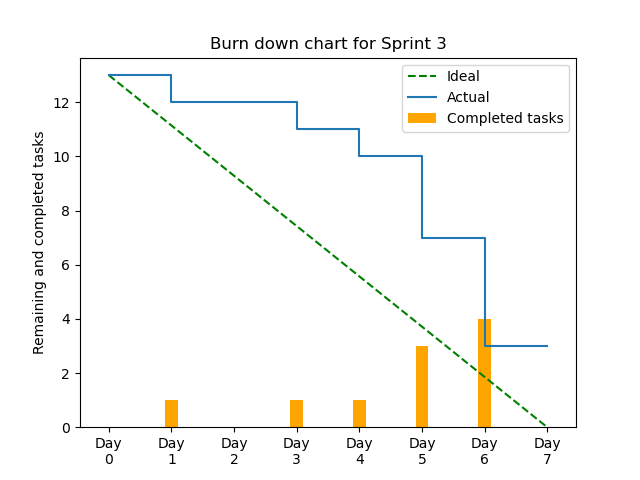
\includegraphics[scale=0.8]{Sprint03_BurnDownChart}
            --- METTERE QUELLO CORRETTO!!! ---

        \end{itemize}
        \newpage
        \subsection{Sprint Retrospective (S02):}
        \begin{itemize}
            \item \textbf{Data:} 15/01/2023
            \newline \textbf{Durata:} 70 min.
            \newline \textbf{Partecipanti:}  \dueP \due
            \newline
            \newline Lo Scrum Master chiede a tutti i membri di evidenziare gli aspetti positivi dello sprint appena concluso. Si evidenzia come una più profonda conoscenza del framework abbia agevolato e velocizzato gli sviluppi e viene confermata l'importanza e i vantaggi dell'approccio Test Driven Design, nonostante l'ingente quantità di effort che richiede. Viene poi proposto un nuovo ordine e dettaglio della Definition of Done (tutti si concorda e viene subito attuato nelle actions di GitHub). Viene proposto di utilizzare la tecnica del "Pair Programming" per agevolare e accellerare l'autonomia dei nuovi sviluppatori. Infine si concorda di utilizzare il metodo "velocity" per la definiziono dello Sprint Backlog, al fine di cercare di organizzare al meglio la pianificazione dello Sprint successivo.
        \end{itemize}

        \newpage

        \section{SPRINT 03}

        \begin{itemize}
            \item Inizio sprint: \textit{22/01/2023}
            \item Fine sprint: \textit{29/01/2023}
        \end{itemize}

        \begin{itemize}
            \item \textbf{Sprint Goal (SG):}
            \begin{indent}
                \newline Il sistema deve permettere all’utente di aggiungere carte da gioco che possiede nella realtà al proprio account e deve permettere all’utente di visualizzare carte da gioco che possiede nella realtà aggiunte al proprio account.
            \end{indent}
        \end{itemize}
        \begin{itemize}
            \item \textbf{Ruoli:}
            \newline \textbf{Product Owner:} Alessio Arcara
            \newline \textbf{Scrum Master:} Matteo Sacco
            \newline \textbf{Development team:} Davide Fermi, Alessia Crimaldi
        \end{itemize}
        \vspace{5mm} %5mm vertical space
        \subsection{Sprint Planning (S03)}
        \textbf{Data:} 22/01/2023
        \newline \textbf{Durata:} 75 min.
        \newline \textbf{Partecipanti:} \treP \tre
        \\
        \newline La riunione inizia con la spiegazione del Product Backlog aggiornato da parte del PO, con definizione delle priorità dei singoli UC. Viene come di consueto applicata la strategia di Poker Planning tra i membri del team, utilizzando come scala la stessa già impiegata nei planning precedenti e con il consueto flusso di planning (stima l'effort per ogni user stories, definizione effort totale settiminale, popolamento dello Sprint Backlog, raffinamento UC e produzione tasks di sviluppo, con stima effort). Come deciso precedentemente, l'approccio di pianificazione per questo nuovo sprint si baserà sulla 'velocity'.
        \newline Come proposto nello Sprint Retrospective, per la durata dello Sprint e in particolar modo nelle fasi iniziali, verrà adottata una strategia di Pair Programming di tipo "Navigator-Driver", al fine di facilitare il passaggio di conoscenza.

        \newpage
        \subsection{Stato Board dopo lo Sprint Planning (S03):}
        \small
        \def\arraystretch{2}%
        \begin{tabular}{ | p{6cm} | p{3.2cm} | p{7.8cm} | p{3cm} | p{2.8cm}| }
            \hline
            \textbf{UC raffinati}
            & \textbf{Product Backlog}
            & \textbf{Sprint Backlog}
            & \textbf{Sprint In progress}
            & \textbf{Sprint Done} \\
            \hline
            \textbf{UC03:} Come visitatore voglio selezionare una carta e vederne i dettagli & &\textbf{Task8 [UC06]\#61:} Creare pagina per visualizzare il mazzo delle possedute (Place, Activity e View) & &
            \textbf{Task1 [UC03]\#16:} Creazione CardView e popolamento delle informazioni \\
            \hline
            \textbf{UC05:} Come utente voglio poter aggiungere le mie carte reali al mazzo delle possedute
            & & \textbf{Task2 [UC05]\#54:} Creare mappa dei mazzi su MapDB & & \\
            \hline
            & & \textbf{Task3 [UC05]\#55:} Modificare RPC signup per aggiungere il mazzo delle possedute alla creazione dell'utente & & \\
            \hline
            & & \textbf{Task4 [UC05]\#56:} Creare RPC per inserire una carta fisica nel mazzo delle possedute dell'utente & & \\
            \hline
            & & \textbf{Task5 [UC05]\#57:} Modificare CardView per poter aggiungere la carta al mazzo delle possedute & & \\
            \hline
            & & \textbf{Task6 [UC05]\#63:} Creare metodo statico in AuthService per controllare validità token e restituire email utente & & \\
            \hline
            & & \textbf{Task7 [UC05]\#71:} Modificare modello PhysicalCard in modo che status sia un valore numerico da 1 a 5 e non una stringa & & \\
            \hline
            \textbf{UC06:} Come utente voglio poter visualizzare il contenuto del mazzo delle possedute
            & & \textbf{Task8 [UC06]\#58:} Creare modello carta fisica che al posto di cardId restituirà sia il titolo della carta che cardId & & \\
            \hline
            & & \textbf{Task8 [UC06]\#59:} Creare RPC per poter visualizzare la lista di carte reali contenute nel mazzo delle possedute & & \\
            \hline
            & & \textbf{Task8 [UC06]\#60:} Inserire hyperlink nel menù laterale (visibile solo se autenticato) & & \\
            \hline
        \end{tabular}
        \newpage

        \subsection{Daily Scrum}

        \begin{itemize}
            \item \textbf{Data:} 23/01/2023
            \newline \textbf{Durata:} 15 min.
            \newline \textbf{Partecipanti:} \tre
            \newline \textbf{Percezione attuale dello SG:} Positiva (Dev 1), Positiva (Dev 2)
        \end{itemize}
        \begin{itemize}
            \item \textbf{Data:} 24/01/2023
            \newline \textbf{Durata:} 15 min.
            \newline \textbf{Partecipanti:} \tre
            \newline \textbf{Percezione attuale dello SG:} Positiva (Dev 1), Positiva (Dev 2)
        \end{itemize}
        \begin{itemize}
            \item \textbf{Data:} 25/01/2023
            \newline \textbf{Durata:} 15 min.
            \newline \textbf{Partecipanti:} \tre
            \newline \textbf{Percezione attuale dello SG:} Tendente al negativo (Dev 1), Positiva (Dev 2)
        \end{itemize}
        \begin{itemize}
            \item \textbf{Data:} 26/01/2023
            \newline \textbf{Durata:} 20 min.
            \newline \textbf{Partecipanti:} \tre
            \newline \textbf{Percezione attuale dello SG:} Positiva (Dev 1), Positiva (Dev 2)
        \end{itemize}
        \begin{itemize}
            \item \textbf{Data:} 27/01/2023
            \newline \textbf{Durata:} 15 min.
            \newline \textbf{Partecipanti:} \tre
            \newline \textbf{Percezione attuale dello SG:} Negativa (Dev 1), Negativa (Dev 2)
        \end{itemize}
        \begin{itemize}
            \item \textbf{Data:} 28/01/2023
            \newline \textbf{Durata:} 15 min.
            \newline \textbf{Partecipanti:} \tre
            \newline \textbf{Percezione attuale dello SG:} Negativa (Dev 1), Negativa (Dev 2)
        \end{itemize}

        \newpage
        \subsection{Stato board dopo finale (S03):}
        \begin{itemize}
            \small
            \def\arraystretch{2}%
            \begin{tabular}{ | p{5cm} | p{3cm} | p{5cm} | p{5cm} | p{5cm}| }
                \hline
                \textbf{UC raffinati}
                & \textbf{Product Backlog}
                & \textbf{Sprint Backlog}
                & \textbf{Sprint In progress}
                & \textbf{Sprint Done} \\
                \hline
                \hline
                \textbf{UC03:} Come visitatore voglio selezionare una carta e vederne i dettagli & & & &
                \textbf{Task1 [UC03]\#16:} Creazione CardView e popolamento delle informazioni \\
                \hline
                \textbf{UC05:} Come utente voglio poter aggiungere le mie carte reali al mazzo delle possedute
                & & & & \textbf{Task2 [UC05]\#54:} Creare mappa dei mazzi su MapDB \\
                \hline
                & & & & \textbf{Task3 [UC05]\#55:} Modificare RPC signup per aggiungere il mazzo delle possedute alla creazione dell'utente \\
                \hline
                & & & & \textbf{Task4 [UC05]\#56:} Creare RPC per inserire una carta fisica nel mazzo delle possedute dell'utente \\
                \hline
                & & & \textbf{Task5 [UC05]\#57:} Modificare CardView per poter aggiungere la carta al mazzo delle possedute & \\
                \hline
                & & & & \textbf{Task6 [UC05]\#63:} Creare metodo statico in AuthService per controllare validità token e restituire email utente \\
                \hline
                & & & & \textbf{Task7 [UC05]\#71:} Modificare modello PhysicalCard in modo che status sia un valore numerico da 1 a 5 e non una stringa \\
                \hline
                \textbf{UC06:} Come utente voglio poter visualizzare il contenuto del mazzo delle possedute
                & & & & \textbf{Task8 [UC06]\#58:} Creare modello carta fisica che al posto di cardId restituirà sia il titolo della carta che cardId \\
                \hline
                & & & \textbf{Task8 [UC06]\#59:} Creare RPC per poter visualizzare la lista di carte reali contenute nel mazzo delle possedute & \\
                \hline
                & &  & & \textbf{Task8 [UC06]\#60:} Inserire hyperlink nel menù laterale (visibile solo se autenticato) \\
                \hline
                & & & \textbf{Task8 [UC06]\#61:} Creare pagina per visualizzare il mazzo delle possedute (Place, Activity e View) & \\
                \hline
            \end{tabular}
        \end{itemize}


        \newpage

        \subsection{Sprint Review (S03)}
        \textbf{Data:} 29/01/2023
        \newline \textbf{Durata:} 95 min.
        \newline \textbf{Partecipanti:} Scrum Master (Matteo Sacco), Product Owner (Alessio Arcara), Dev 1 (Alessia Crimaldi), Dev 2 (Davide Fermi)
        \newline Viene prima effettuata la demo da parte dei developers. Il PO decide di non rilasciare viste le poche funzionalit\'a aggiunte rispetto alla precedente versione: si considera fallito lo sprint.
        \newline Nella sprint review vengono evidenziati soprattutto problemi nella difficolt\'a di scrivere il codice da parte dei developers all'interno di un progetto cos\'{\i} fortemente strutturato. Allo stesso modo \'e messo in risalto che il TDD risulta a volte quasi bloccante, soprattutto quando si rende necessario creare molti mock da passare nei test. Inoltre viene fatto presente che durante la settimana si sono resi necessari diversi refactor rispetto a pattern e modelli scelti in precedenza, i quali per\'o non hanno rallentato i developers poich\'e non impattanti sui task che stavano sviluppando. Viene evidenziata una problematica legata al GsonSerializer e analizzate tre diverse proposte per la risoluzione del problema.
        \newline Si concorda che spesso si sono travisati gli obiettivi definiti nei task, andando ad ampliare le funzionalit\'a descritte perch\'e ritenute troppo poche e troppo semplici; questo ha consistito in una complicazione 'auto imposta' dai developers.
        \newline

        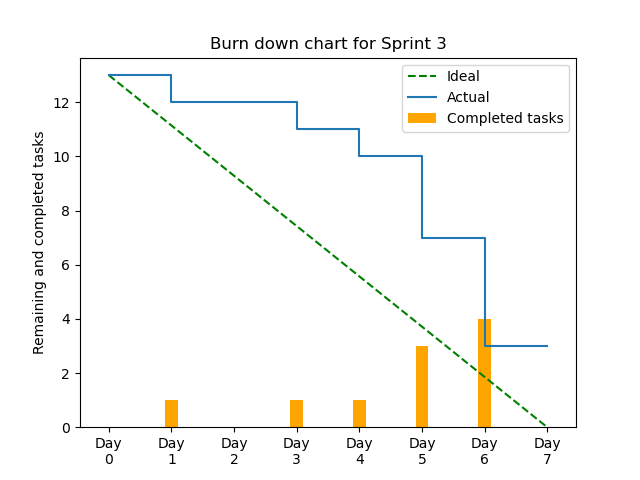
\includegraphics[scale=0.8]{Sprint03_BurnDownChart}

        \newpage
        \subsection{Sprint Retrospective (S03):}
        \textbf{Data:} 29/01/2023
        \newline \textbf{Durata:} 45 min.
        \newline \textbf{Partecipanti:} Scrum Master (Matteo Sacco), Product Owner (Alessio Arcara), Dev 1 (Alessia Crimaldi), Dev 2 (Davide Fermi)
        \newline Si concorda che l'approccio TDD risulta efficiente soprattutto nel fare refactor del codice, quindi si decide di proseguire con questa metodologia, nonostante il costo iniziale. Inoltre si decide di continuare a fare Pair Programming e di introdurre in parte minore anche XP, poich\'e si \'e rivelato utile negli ultimi giorni di Sprint per fare il refactor di alcune porzioni di codice estese.
        \newline Si concorda che l'approccio di Pair Programming nella fase iniziale dello Sprint ha contribuito in modo significativo alla velocizzazione sia di produzione di codice per i nuovi developer, che di diffusione della conoscenza acquisita.
        \newline Viene ridiscusso l'ordine di dettaglio della Definition of Done. e viene concordato che la chiusura della Documentazione sarà spostata prima dell'accettazione della PR. Questo perch\'e durante la settimana \'e stato introdotto uno strumento per creare in automatico il Burndown Chart il quale riconosce come chiuso il task dopo che la PR \'e stata accettata.
        \newpage
            \end{landscape}
\end{document}
